\chapter{Diseño de recursos distribuidos específicos}
\label{cap:disenyo}


%%%%%%%%%%%%%%%%%%%%%%%%%%%%%%%%%%%%%%%%%%%%%%%%%%%%%%%%%%%%%%%%%%%%%%%%%%%%%%%%
\section{Diseño y uso de un recurso distribuido para una infraestructura AppScale}

Una infraestructura AppScale puede ser definida de dos maneras: mediante un despliegue por defecto o uno personalizado. En un despliegue por defecto un nodo es el encargado de controlar la infraestructura y el resto de nodos se encargan de hacer el resto del trabajo. En un despliegue personalizado podemos especificar con mayor grado de precisión qué tipo de trabajo debe hacer cada nodo. Por ejemplo, podemos indicar qué nodos se encargarán de alojar las aplicaciones de los usuarios, qué nodos alojarán la base de datos o qué nodos serán los encargados de ejecutar los trabajos de computación. Para administrar una infraestructura AppScale, sin importar el tipo de despliegue, necesitaremos una cuenta de correo y una contraseña. Este usuario y contraseña son necesarios para poder administrar las aplicaciones alojadas y observar el estado de la infraestructura.

\subsection{Manifiesto de recurso distribuido}

La sintaxis del manifiesto distribuido no se verá afectada por los dos tipos de despliegue posibles, pero sí que tendrá que reflejar los parámetros necesarios para realizar las tareas de administración de la infraestructura. Éste podría ser un ejemplo de un manifiesto para la puesta en marcha de una infraestructura de tipo AppScale:

\begin{lstlisting}
appscale {'mycloud':
   ip_file      => "/etc/puppet/modules/appscale/files/appscale-ip.yaml",
   img_file     => "/etc/puppet/modules/appscale/files/appscale-img.yaml",
   domain       => "/etc/puppet/modules/appscale/files/mycloud-template.xml",
   pool         => ["155.210.155.70"],
   app_email    => "user@mail.com"
   app_password => "password"
   ensure       => running,
}
\end{lstlisting}

La parada de una infraestructura AppScale es más sencilla, y por tanto también lo es su manifiesto:

\begin{lstlisting}
appscale {'mycloud':
   pool   => ["155.210.155.70"],
   ensure => stopped,
}
\end{lstlisting}

\subsection{Fichero de roles}

El fichero de roles sí que debe reflejar los dos posibles tipos de despliegue. En un despliegue por defecto los posibles roles que puede tomar un nodo son:

\begin{description}
\item[\texttt{controller}]: La máquina que desempeñará el rol de nodo controlador.
\item[\texttt{servers}]: La lista de máquinas que desempeñarán el rol de nodos de trabajo.
\end{description}

Un fichero de roles para este despliegue sería de esta forma:

\begin{yamlcode}
--- 
:controller: 155.210.155.73
:servers: 
- 155.210.155.177
- 155.210.155.178
\end{yamlcode}

Por otra parte, los posibles roles que puede desempeñar un nodo en un despliegue personalizado y que resultan interesantes desde nuestro punto de vista son:

\begin{description}
\item[\texttt{master}]: La máquina que desempeñará el rol de nodo maestro.
\item[\texttt{appengine}]: Los servidores para alojar las aplicaciones.
\item[\texttt{database}]: Las máquinas que contienen la base de datos.
\item[\texttt{login}]: La máquina encargada de redirigir a los usuarios a sus servidores. Es también la que se le facilita al administrador de la infraestructura para que realice las tareas administrativas.
\item[\texttt{open}]: Las máquinas de ejecución de trabajos. También pueden ser usadas como nodos de reserva por si falla algún otro nodo.
\end{description}

\begin{figure} [!htbp]
  \centering
  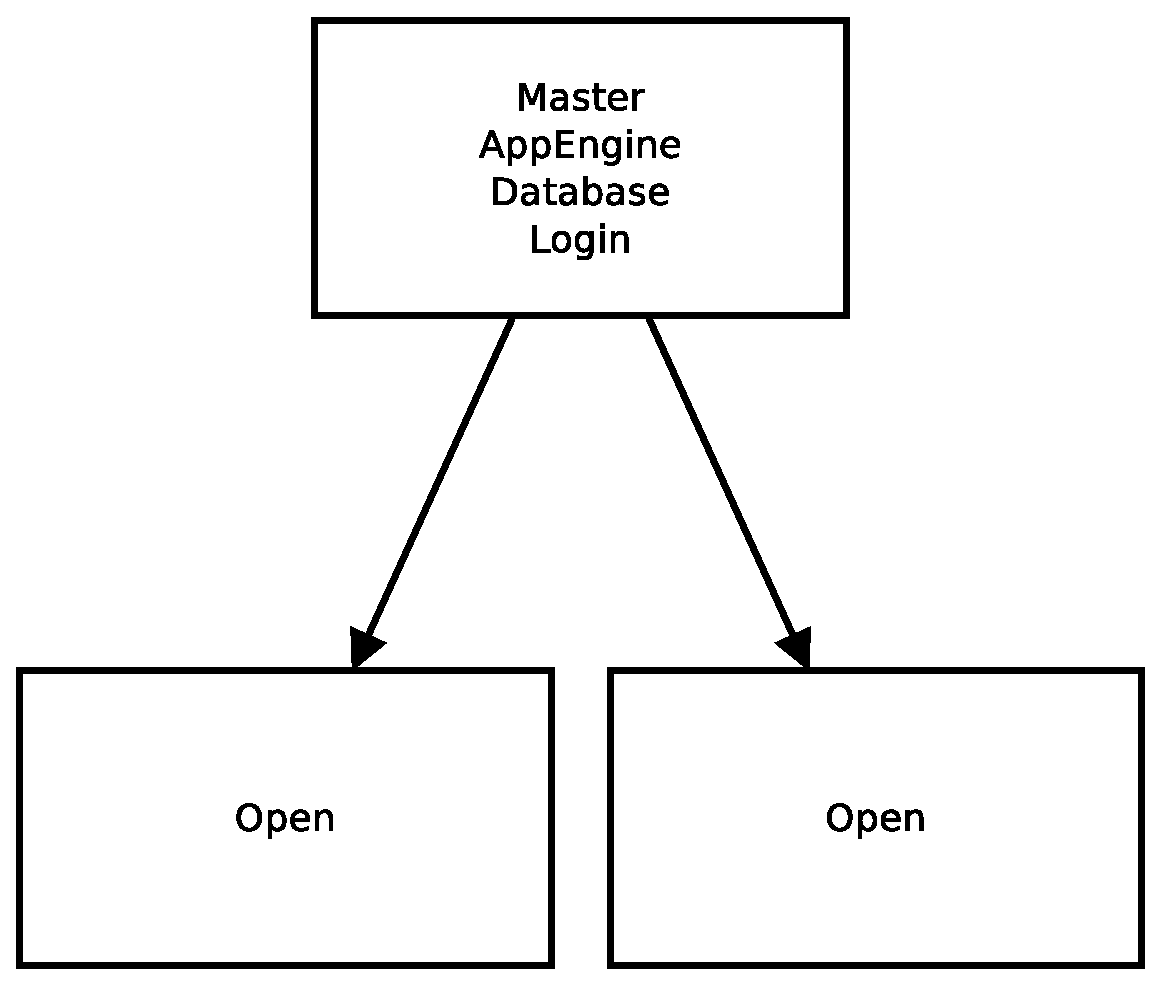
\includegraphics[width=0.5\textwidth]{figuras/Arquitectura_AppScale.eps}
  \caption{Infraestructura AppScale en despliegue personalizado.}
\label{figure:arquitectura-appscale}
\end{figure}

Hay multitud de despliegues posibles combinando estos roles, pero será de especial interés para nosotros el que permite ejecutar trabajos de computación en AppScale (Figura \ref{figure:arquitectura-appscale}). Un despliegue de este tipo podría conseguirse con un fichero similar a éste:

\begin{yamlcode}
---
:master:    155.210.155.73
:appengine: 155.210.155.73
:database:  155.210.155.73
:login:     155.210.155.73
:open:
- 155.210.155.177
- 155.210.155.178
\end{yamlcode}


%%%%%%%%%%%%%%%%%%%%%%%%%%%%%%%%%%%%%%%%%%%%%%%%%%%%%%%%%%%%%%%%%%%%%%%%%%%%%%%%
\section{Diseño y uso de un recurso distribuido para una infraestructura Torque}

Una infraestructura Torque está formada por un nodo maestro y un conjunto de nodos de computación (Figura \ref{figure:arquitectura-torque}). El nodo maestro es el encargado de recibir los trabajos a ejecutar y de asegurar una correcta planificación para esos trabajos; en su versión más simple el planificador es una cola FIFO. Los nodos de computación son los encargados de ejecutar los trabajos enviados por el nodo maestro y, una vez terminados, enviarle los resultados de vuelta.

\begin{figure} [!htbp]
  \centering
  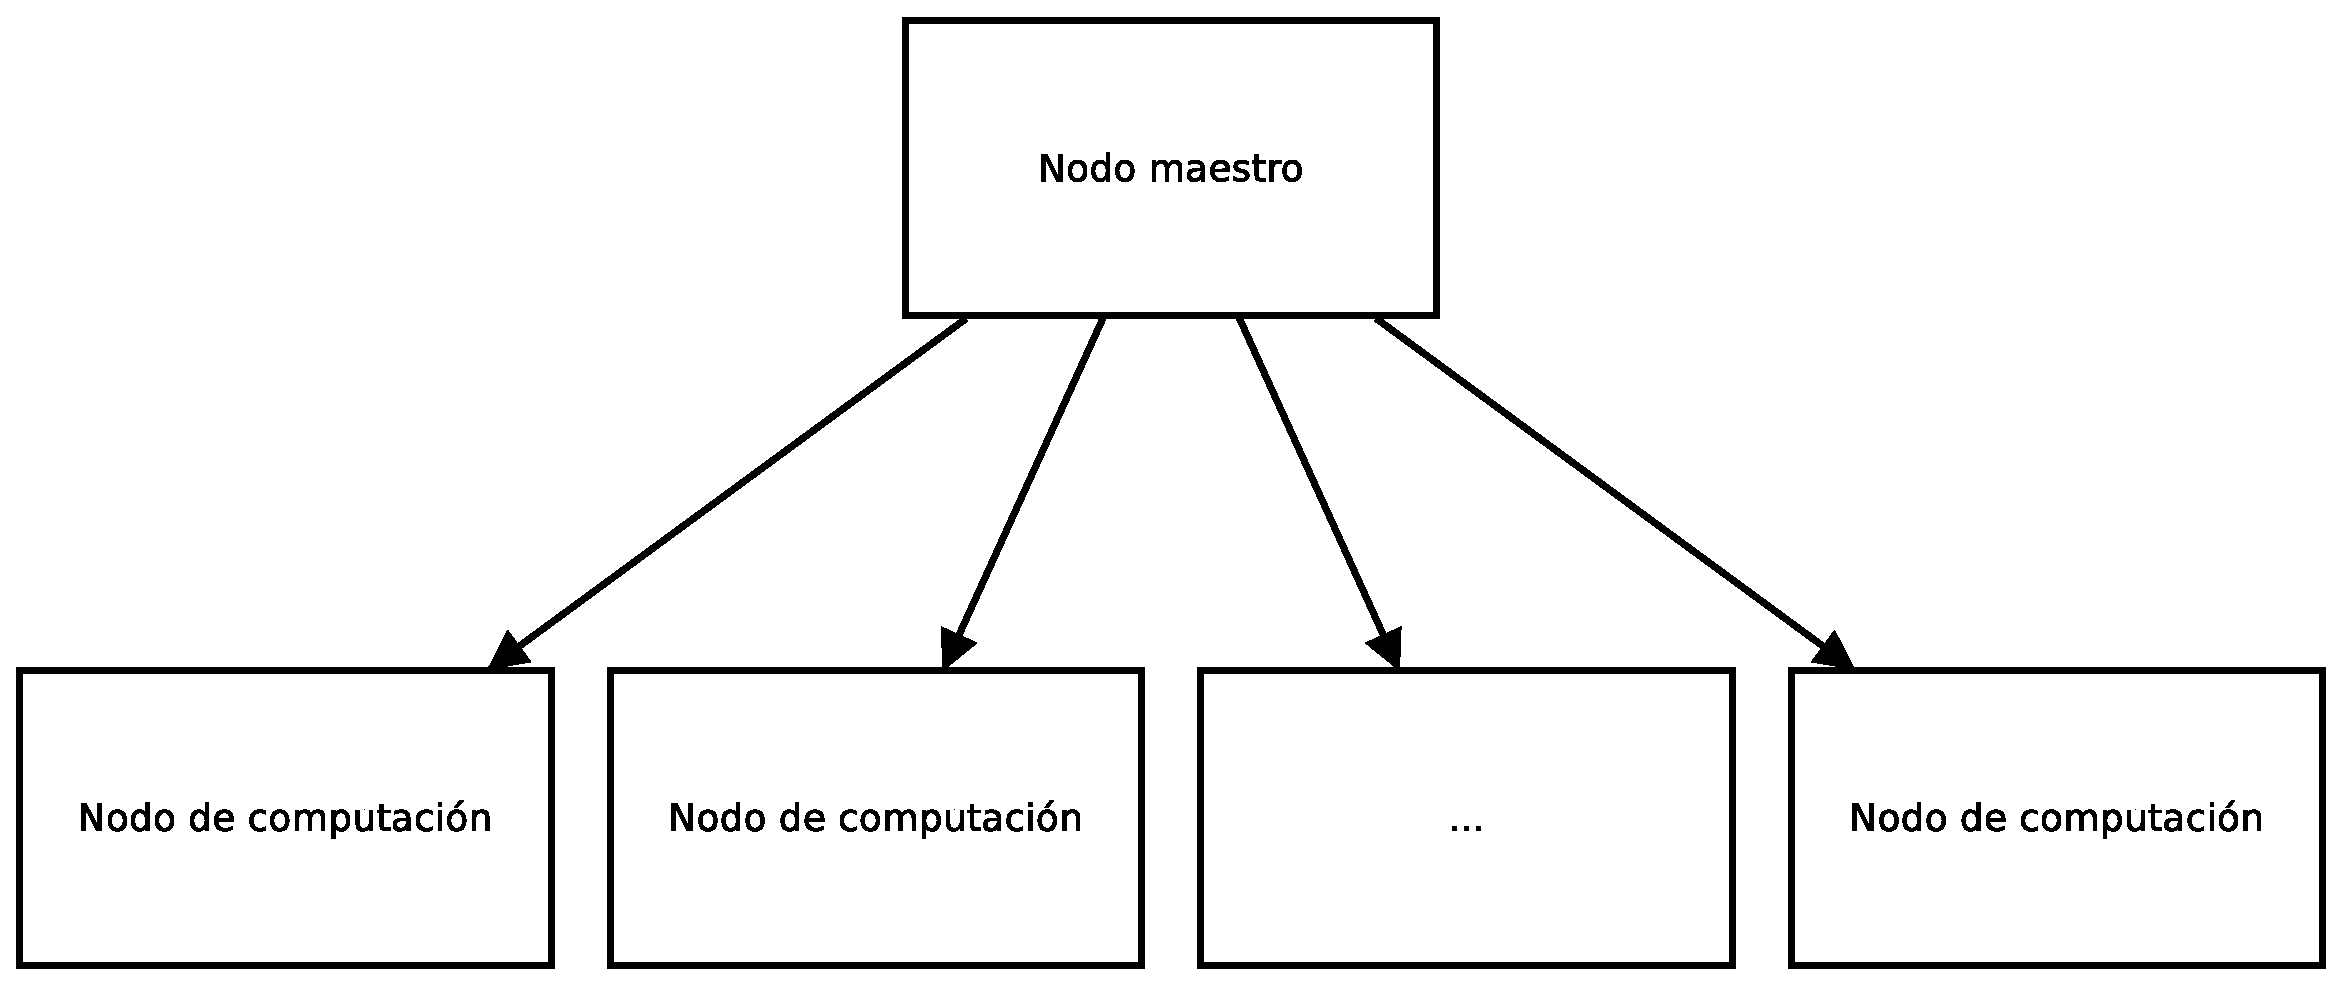
\includegraphics[width=13.5cm]{figuras/Arquitectura_Torque.eps}
  \caption{Infraestructura Torque.}
\label{figure:arquitectura-torque}
\end{figure}

\subsection{Manifiesto de recurso distribuido}

La sintaxis del manifiesto distribuido es similar a la usada en el ejemplo de AppScale, sólo que aquí no aparecen los parámetros de administración que aparecían en aquél, ya que Torque no requiere su uso. Un ejemplo para la puesta en marcha de una infraestructura Torque sería similar a éste:

\begin{lstlisting}
torque {'mycloud':
   ip_file  => "/etc/puppet/modules/torque/files/jobs-ip.yaml",
   img_file => "/etc/puppet/modules/torque/files/jobs-img.yaml",
   domain   => "/etc/puppet/modules/torque/files/mycloud-template.xml",
   pool     => ["155.210.155.70"],
   ensure   => running,
}
\end{lstlisting}

En este caso, la parada de la infraestructura es algo más compleja que en el ejemplo de AppScale. Un posible manifiesto de parada sería similar a éste:

\begin{lstlisting}
torque {'mycloud':
   ip_file  => "/etc/puppet/modules/torque/files/jobs-ip.yaml",
   img_file => "/etc/puppet/modules/torque/files/jobs-img.yaml",
   pool     => ["155.210.155.70"],
   ensure   => stopped,
}
\end{lstlisting}

\subsection{Fichero de roles}

El contenido del fichero de roles sí que será más sencillo que en el caso de AppScale, ya que en Torque tenemos únicamente los roles de nodo maestro y nodo de computación. La especificación completa de la sintaxis es la siguiente:

\begin{description}
\item[\texttt{head}]: La máquina que desempeñará el rol de nodo maestro.
\item[\texttt{compute}]: La lista de máquinas que desempeñarán el rol de nodos de computación.
\end{description}

Un fichero de especificación de roles para una infraestructura Torque tendría un contenido similar a éste:
\begin{yamlcode}
--- 
:head: 155.210.155.73
:compute:
- 155.210.155.177
- 155.210.155.178
\end{yamlcode}


%%%%%%%%%%%%%%%%%%%%%%%%%%%%%%%%%%%%%%%%%%%%%%%%%%%%%%%%%%%%%%%%%%%%%%%%%%%%%%%%
\section{Diseño y uso de un recurso distribuido para una infraestructura web de tres niveles}

Una típica arquitectura de servicios web consta de al menos tres niveles: balanceo de carga, servidores web y base de datos. Cada uno de estos niveles está compuesto por al menos un elemento clave: el balanceador de carga, el servidor web y el servidor de base de datos, respectivamente. El balanceador de carga es el punto de entrada al sistema y el que se encarga, como su nombre indica, de repartir las peticiones de los clientes a los distintos servidores web. Los servidores web se encargan de servir las páginas web a los clientes y para ello, dependiendo de las peticiones que hagan los clientes, podrán leer o almacenar información en la base de datos. Para manipular dicha información los servidores web tendrán que comunicarse con el servidor de base de datos, que es el que hará efectiva la lectura y modificación de la información.\\

\begin{figure} [!htbp]
  \centering
  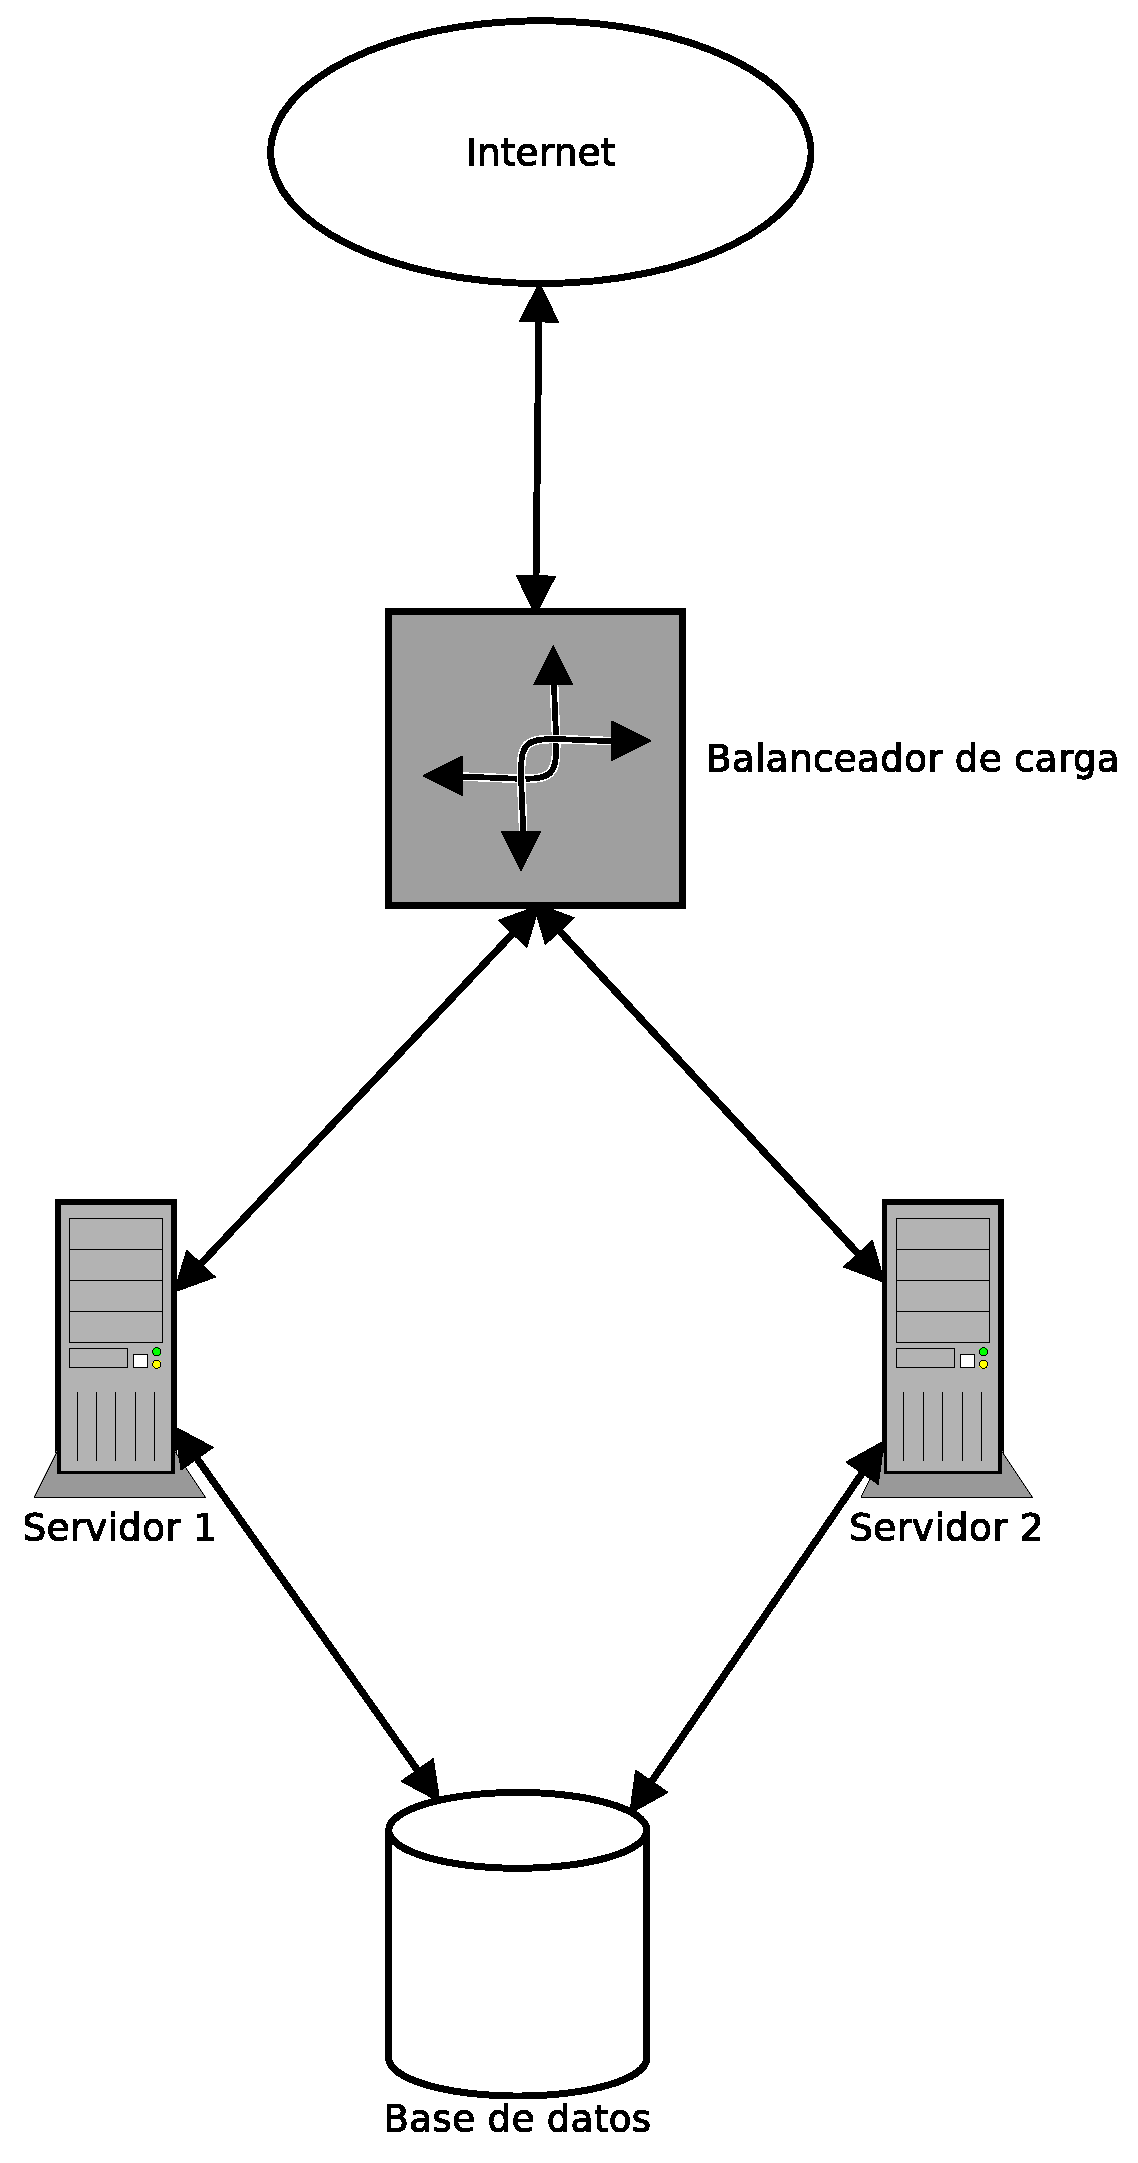
\includegraphics[width=0.5\textwidth]{figuras/Arquitectura_web2.eps}
  \caption{Infraestructura web de tres niveles.}
\label{figure:arquitectura-web}
\end{figure}

Para demostrar la validez del modelo desarrollado se verá como, además de sobre las infraestructuras AppScale y Torque, también se puede aplicar dicho modelo sobre una infraestructura que no tiene nada que ver con la ejecución de trabajos: una infraestructura de servicios web. En el ejemplo se ha validado una infraestructura que consta de un balanceador de carga, dos servidores web y un servidor de bases de datos (Figura \ref{figure:arquitectura-web}).

%%% Revisar
%%% Como balanceador de carga se ha usado nginx y como servidor de base de datos se ha usado MySQL. La creación de la página web se ha hecho usando el framework Sinatra sobre el servidor web WEBrick. Todos ellos corren sobre máquinas con sistema operativo Ubuntu.\\

\subsection{Manifiesto de recurso distribuido}

La sintaxis del manifiesto de puesta en marcha es fundamentalmente similar a la utilizada en el ejemplo de Torque, ya que tampoco en este caso tenemos parámetros de administración de la infraestructura. Así pues, si se quiere poner en marcha una infraestructura web de tres niveles podemos usar un manifiesto similar a éste:

\begin{lstlisting}
web {'mycloud':
   ip_file  => "/etc/puppet/modules/web/files/web-ip.yaml",
   img_file => "/etc/puppet/modules/web/files/web-img.yaml",
   domain   => "/etc/puppet/modules/web/files/mycloud-template.xml",
   pool     => ["155.210.155.70"],
   ensure   => running,
}
\end{lstlisting}

En este caso, el manifiesto de parada vuelve a ser sencillo. Un posible ejemplo es éste:

\begin{lstlisting}
web {'mycloud':
   pool   => ["155.210.155.70"],
   ensure => stopped,
}
\end{lstlisting}

\subsection{Fichero de roles}

El contenido del fichero de especificación de roles sí que poseerá valores distintos a los que tenía cualquiera de los dos ejemplos anteriores ya que estamos describiendo una infraestructura distinta. Los roles que pueden desempeñar los nodos dentro de una infraestructura web son:
\begin{description}
\item[\texttt{balancer}]: La máquina que desempeñará el rol de balanceador de carga.
\item[\texttt{server}]: La lista de máquinas que desempeñarán el rol de servidor web.
\item[\texttt{database}]: La máquina que desempeñará el rol de servidor de base de datos.
\end{description}

Un ejemplo completo del fichero de especificación de roles tendría un contenido similar a éste:
\begin{yamlcode}
--- 
:balancer: 155.210.155.175
:server:
- 155.210.155.73
- 155.210.155.178
:database: 155.210.155.177
\end{yamlcode}
